\chapter{Periodicity and Photonic Bands}
\label{ch:periodicity}

\begin{chapterlead}
A homogeneous dielectric has a continuous spectrum: any frequency can
propagate. Introduce a periodic modulation of the permittivity and the
spectrum reorganizes into bands separated by gaps---frequency windows in
which no propagating mode exists. The band structure of photonic
crystals is derived directly from the Maxwell eigenproblem of
Chapter~\ref{ch:light-eigenvalue}, using Bloch's theorem as the organizing
principle. The real, orthogonal, gapped band structure established here is
the Hermitian baseline against which all non-Hermitian modifications in
later chapters will be measured.
\end{chapterlead}


%% ================================================================
\section{Periodic permittivity and the direct lattice}
\label{sec:periodic-eps}

Consider a medium whose relative permittivity is periodic:
\begin{equation}
 \epsr(\rr + \mathbf{R}) = \epsr(\rr)
 \qquad\text{for all lattice vectors}\quad
 \mathbf{R} = n_1\mathbf{a}_1 + n_2\mathbf{a}_2 + n_3\mathbf{a}_3,
 \label{eq:periodic-eps}
\end{equation}
where $\mathbf{a}_1, \mathbf{a}_2, \mathbf{a}_3$ are primitive lattice
vectors and $n_i \in \mathbb{Z}$. We assume $\epsr(\rr)$ is real,
positive, and bounded, so the self-adjointness results of
Chapter~\ref{ch:energy-inner} apply within each unit cell.

The set of all lattice vectors $\mathbf{R}$ forms the \emph{direct
lattice}. The primitive unit cell $\Omega_{\mathrm{uc}}$ can be chosen
as the parallelotope spanned by $\{\mathbf{a}_i\}$ or, more symmetrically,
as the Wigner--Seitz cell centered on a lattice point.

For most of this chapter we work in two dimensions, where the permittivity
$\epsr(x,y)$ is periodic in the $(x,y)$ plane and uniform along $z$.
This covers ideal two-dimensional photonic crystals---arrays of dielectric
rods or air holes uniform along the third direction---and gives a useful
starting point for slab photonic crystals when vertical confinement can be
treated separately. It also allows the TE/TM decomposition of
Section~\ref{sec:2d-reductions}. The extension to fully three-dimensional
crystals is conceptually straightforward but notationally heavier;
see~\cite{paz2019tutorial} for explicit three-dimensional calculations.


%% ================================================================
\section{Reciprocal lattice and Brillouin zone}
\label{sec:reciprocal}

The \emph{reciprocal lattice} is defined by vectors $\GG$ satisfying
$e^{i\GG\cdot\mathbf{R}} = 1$ for all direct-lattice vectors $\mathbf{R}$.
In two dimensions, the primitive reciprocal-lattice vectors
$\mathbf{b}_1, \mathbf{b}_2$ satisfy
\begin{equation}
 \mathbf{a}_i \cdot \mathbf{b}_j = 2\pi\,\delta_{ij},
 \qquad i,j = 1,2.
 \label{eq:reciprocal-vectors}
\end{equation}
The first \emph{Brillouin zone} (BZ) is the Wigner--Seitz cell of the
reciprocal lattice. It is the fundamental domain for the wave vector
$\kk$: any $\kk$ outside the first BZ can be mapped back into it by
subtracting a reciprocal-lattice vector.

\begin{example}[Square and triangular lattices]
For a square lattice with period $a$, the primitive vectors are
$\mathbf{a}_1 = a\hat{x}$, $\mathbf{a}_2 = a\hat{y}$, and the
reciprocal-lattice vectors are $\mathbf{b}_1 = (2\pi/a)\hat{x}$,
$\mathbf{b}_2 = (2\pi/a)\hat{y}$. The first BZ is a square of side
$2\pi/a$ centered at the origin.

For a triangular lattice with $\mathbf{a}_1 = a\hat{x}$,
$\mathbf{a}_2 = a(\hat{x}/2 + \sqrt{3}\hat{y}/2)$, the BZ is a regular
hexagon. Its high-symmetry points---$\Gamma$, $M$, $K$---play a
central role in photonic-crystal band diagrams.
\end{example}

Figure~\ref{fig:ch3-reciprocal-lattice-bz} fixes the reciprocal-space
geometry that will be used throughout the chapter. The important point is
not the artistic shape of the cell, but the convention: the first BZ is a
Wigner--Seitz cell of the reciprocal lattice, and the red curves are
standard high-symmetry paths used to display bands.

\begin{figure}[t]
 \centering
 
\includegraphics[width=0.94\linewidth]{fig_f3_reciprocal_lattice_bz.pdf}
 \caption{First Brillouin zones and standard high-symmetry paths in two
 common two-dimensional lattices. (a) For the square lattice the axes are
 $k_x a/\pi$ and $k_y a/\pi$; the first BZ is the square
 $[-1,1]^2$, and the red path is $\Gamma$--$X$--$M$--$\Gamma$.
 (b) For the triangular lattice the first BZ is hexagonal. The axes are
 normalized by $|G_{\mathrm{nn}}|/2$, where $G_{\mathrm{nn}}$ is a nearest
 reciprocal-lattice vector. In this convention the $K$-type points are
 the hexagon corners at radius $2/\sqrt{3}$, the $M$-type points are edge
 midpoints at radius $1$, and the red curve shows one
 $\Gamma$--$M$--$K$--$\Gamma$ sector. The two panels therefore use their
 natural reciprocal-space normalizations rather than a common length scale.}
 \label{fig:ch3-reciprocal-lattice-bz}
\end{figure}

Because $\epsr(\rr)$ is periodic, it admits a Fourier expansion:
\begin{equation}
 \epsr(\rr) = \sum_{\GG} \hat{\eps}_{\GG}\,e^{i\GG\cdot\rr},
 \label{eq:fourier-eps}
\end{equation}
where the sum runs over all reciprocal-lattice vectors and the Fourier
coefficients are
\begin{equation}
 \hat{\eps}_{\GG}
 = \frac{1}{|\Omega_{\mathrm{uc}}|}
 \int_{\Omega_{\mathrm{uc}}} \epsr(\rr)\,e^{-i\GG\cdot\rr}\;\dd^2 r.
 \label{eq:fourier-coeffs}
\end{equation}
The reality of $\epsr$ implies
$\hat{\eps}_{-\GG} = \hat{\eps}_{\GG}^*$.

\subsection{The dielectric scaling law}
\label{ssec:dielectric-scaling}

The Maxwell eigenproblem possesses a scaling property with no counterpart
in the Schr\"odinger equation. If $\epsr(\rr)$ describes a photonic crystal
with lattice constant~$a$, then the rescaled medium
$\epsr'(\rr) = \epsr(\rr/s)$ with lattice constant~$sa$ has eigenfrequencies
$\omega_n'(\kk') = \omega_n(\kk)/s$ at wave vectors $\kk' = \kk/s$.
The band structure scales inversely with the lattice constant, with no
change in shape:
\begin{equation}
 \frac{\omega_n(\kk)\,a}{2\pi c}
 = \frac{\omega_n'(\kk')\,(sa)}{2\pi c}.
 \label{eq:dielectric-scaling}
\end{equation}
This follows because the curl operator $\nabla\times$ scales as $1/a$
and the eigenvalue $\omega^2/c^2$ scales as $1/a^2$, while $\epsr$ is
dimensionless and unchanged by the spatial rescaling.

The scaling law has two practical consequences. First, band diagrams
are conventionally plotted in dimensionless units: the frequency axis is
$\omega a/(2\pi c)$ and the wave-vector axis is $ka/\pi$.
A single dimensionless band diagram then covers all physical lattice
constants simultaneously. Second, a photonic crystal designed at microwave
frequencies can be scaled to the optical regime simply by shrinking the
lattice constant, provided the material dispersion of $\epsr$ at the new
frequency is accounted for. This scale-free property is unique to
Maxwell's equations: the Schr\"odinger equation possesses a fundamental
length (the Bohr radius) set by $\hbar$, $m$, and $e$, so electronic
band structures do not rescale in this way.

The dimensionless presentation also clarifies the role of the dielectric
contrast $\varepsilon_{\max}/\varepsilon_{\min}$: it is the only
parameter (together with the geometry) that controls the dimensionless
band structure. Increasing the contrast widens all gaps simultaneously,
while changing the lattice constant merely shifts the physical frequency
scale.


%% ================================================================
\section{Bloch's theorem for Maxwell fields}
\label{sec:bloch-theorem}

The Maxwell curl--curl operator $\Mop$ defined in~\eqref{eq:maxwell-op-H}
commutes with the discrete translation operator
$T_{\mathbf{R}}\HH(\rr) = \HH(\rr + \mathbf{R})$, because
$\epsr(\rr + \mathbf{R}) = \epsr(\rr)$. Since $\Mop$ and
$\{T_{\mathbf{R}}\}$ share a common set of eigenstates, the eigenmodes of
$\Mop$ can be chosen to be simultaneous eigenstates of all lattice
translations:
\begin{equation}
 T_{\mathbf{R}}\,\HH_{n\kk}(\rr)
 = e^{i\kk\cdot\mathbf{R}}\,\HH_{n\kk}(\rr).
 \label{eq:bloch-condition}
\end{equation}
This is \emph{Bloch's theorem}. It states that each eigenmode can be
written as
\begin{equation}
 \boxed{
 \HH_{n\kk}(\rr) = e^{i\kk\cdot\rr}\,\mathbf{u}_{n\kk}(\rr),
 }
 \label{eq:bloch-mode}
\end{equation}
where $\mathbf{u}_{n\kk}(\rr)$ is a vector function with the periodicity
of the lattice: $\mathbf{u}_{n\kk}(\rr + \mathbf{R}) = \mathbf{u}_{n\kk}(\rr)$.

The band index $n = 1, 2, 3, \ldots$ labels the discrete eigenvalues at each
$\kk$, and $\kk$ is a continuous label running over the first Brillouin zone.
The eigenfrequency $\omega_n(\kk)$ as a function of $\kk$ is the
\emph{$n$-th photonic band}.

\begin{booknote}[Bloch's theorem is a consequence of symmetry]
The derivation above used only two ingredients: (i)~the operator $\Mop$
commutes with discrete translations, and (ii)~the translation operators
form an abelian group whose irreducible representations are one-dimensional
and labeled by $\kk$. No specific form of $\epsr$ was assumed beyond
periodicity. This means Bloch's theorem holds equally for the $\EE$-field
formulation, for magnetic media, and---crucially for later chapters---for
complex $\epsr$, as long as the periodicity is maintained. In the
non-Hermitian case, Bloch's theorem still provides a labeling by $\kk$,
but the eigenfrequencies become complex and the orthogonality of Bloch
modes fails.
\end{booknote}


%% ================================================================
\section{The unit-cell eigenproblem}
\label{sec:unit-cell}

Substituting the Bloch form~\eqref{eq:bloch-mode} into the Maxwell
eigenproblem $\Mop\HH = (\omega^2/c^2)\HH$ transforms the problem on
all of space into a problem on a single unit cell. Define the
$\kk$-dependent operator
\begin{equation}
 \Mop_\kk\,\mathbf{u}
 = (\nabla + i\kk)\times
 \left[\frac{1}{\epsr(\rr)}
 (\nabla + i\kk)\times\mathbf{u}\right],
 \label{eq:theta-k}
\end{equation}
which acts on periodic vector fields $\mathbf{u}(\rr)$ defined on
$\Omega_{\mathrm{uc}}$ with periodic boundary conditions. The eigenvalue
equation becomes
\begin{equation}
 \Mop_\kk\,\mathbf{u}_{n\kk}
 = \frac{\omega_n(\kk)^2}{c^2}\,\mathbf{u}_{n\kk},
 \label{eq:unit-cell-evp}
\end{equation}
with $\mathbf{u}_{n\kk}$ subject to periodic boundary conditions on
$\partial\Omega_{\mathrm{uc}}$.

The operator $\Mop_\kk$ is self-adjoint on the unit cell for real
$\epsr > 0$, because the surface terms from integration by parts cancel
between opposite faces (the Bloch phase factors have been absorbed into
$\nabla + i\kk$, and the boundary conditions are now strictly periodic).
Consequently, for each $\kk$ the eigenvalues
$\omega_n(\kk)^2/c^2$ are real and non-negative, the eigenfunctions
$\mathbf{u}_{n\kk}$ are orthogonal, and all the results of
Chapter~\ref{ch:energy-inner} apply with $\Mop$ replaced by $\Mop_\kk$.

The unit-cell eigenproblem~\eqref{eq:unit-cell-evp} is the starting point
for all numerical photonic band calculations. The standard approach
is to expand $\mathbf{u}_{n\kk}$ and $\epsr^{-1}$ in plane waves
(reciprocal-lattice vectors $\GG$), converting the differential equation
into a matrix eigenvalue problem that is solved for each $\kk$ on a
discrete grid in the Brillouin zone~\cite{paz2019tutorial}.


%% ================================================================
\section{One-dimensional photonic crystals}
\label{sec:1d-photonic-crystal}

Before treating two-dimensional systems, it is instructive to solve the
simplest photonic crystal exactly: a one-dimensional stack of alternating
dielectric layers. This example makes band gaps, Bloch wave vectors, and
the connection between the Maxwell eigenproblem and scattering theory
completely explicit.

\subsection{Transfer matrix for a bilayer}
\label{ssec:bilayer-transfer-ch3}

Consider a periodic stack along~$x$ with unit cell consisting of a layer
of thickness~$d_A$ and refractive index $n_A = \sqrt{\varepsilon_A}$
followed by a layer of thickness~$d_B$ and refractive index
$n_B = \sqrt{\varepsilon_B}$, so the period is $a = d_A + d_B$.
For normal incidence, the tangential field vector may be written as
$(E,\eta_0 H)^\transpose$, where the magnetic field is scaled by the
vacuum impedance. Its value at one side of the unit cell is related to
the value at the other side by a $2\times 2$ characteristic matrix~$M$:
\begin{equation}
 \begin{pmatrix} E_{m+1} \\ \eta_0 H_{m+1} \end{pmatrix}
 = M \begin{pmatrix} E_m \\ \eta_0 H_m \end{pmatrix},
 \qquad
 M = M_B \, M_A,
 \label{eq:1d-transfer}
\end{equation}
where the single-layer transfer matrix is
\begin{equation}
 M_j = \begin{pmatrix}
 \cos\phi_j & -i\sin\phi_j / n_j \\
 -i\,n_j\sin\phi_j & \cos\phi_j
 \end{pmatrix},
 \qquad
 \phi_j = \frac{\omega\,n_j\,d_j}{c},
 \label{eq:single-layer-transfer}
\end{equation}
for $j = A, B$. The phase $\phi_j$ is the optical path length through
layer~$j$ measured in radians. This transfer matrix is unimodular,
$\det M_j = 1$, as required by energy conservation in a lossless medium.
The product $M = M_B\,M_A$ is therefore also unimodular.

\subsection{Bloch condition and the dispersion relation}
\label{ssec:1d-dispersion}

Bloch's theorem requires that traversing one period multiplies the field
amplitudes by $e^{iKa}$, where $K$ is the Bloch wave vector. This means
$M$ has eigenvalue $e^{iKa}$, so
\begin{equation}
 \boxed{
 \cos(Ka) = \tfrac{1}{2}\operatorname{tr} M
 = \cos\phi_A\cos\phi_B
 - \tfrac{1}{2}\!\left(\frac{n_A}{n_B} + \frac{n_B}{n_A}\right)
 \sin\phi_A\sin\phi_B.
 }
 \label{eq:1d-dispersion-ch3}
\end{equation}
This is the exact photonic dispersion relation for a 1D periodic stack.
When $|\tfrac{1}{2}\operatorname{tr} M| \le 1$, the Bloch wave vector
$K$ is real and a propagating Bloch mode exists: these frequencies lie
in a \emph{pass band}. When $|\tfrac{1}{2}\operatorname{tr} M| > 1$,
$K$ acquires an imaginary part and the wave is evanescent: these
frequencies lie in a \emph{stop band} or band gap.

It is convenient to define the \emph{half-trace}
\begin{equation}
 \xi(\omega) \;\equiv\; \tfrac{1}{2}\operatorname{tr}M(\omega),
 \label{eq:half-trace-def}
\end{equation}
so that the pass-band condition is simply $|\xi|\le 1$.
The band structure is found by solving
$K(\omega) = \arccos[\xi(\omega)]/a$.
The result is a set of bands separated by gaps, plotted as $\omega$ versus
$K$ or equivalently as $K$ versus~$\omega$. When the two materials become
identical ($n_A = n_B$), the trace reduces to
$\cos(\omega a\,n/c)$ and the bands become the free-photon dispersion
folded into the first Brillouin zone, with no gaps.

The same trace formula is shown in Figure~\ref{fig:ch3-1d-transfer-bands}
for a representative high-contrast bilayer. This figure is deliberately
plotted in two equivalent ways: as pass bands in the reduced zone and as the
half-trace criterion. It is the inequality $|\xi(\omega)|\leq 1$, not the
visual shading, that defines a propagating Bloch wave.

\begin{figure}[t]
 \centering
 
\includegraphics[width=0.94\linewidth]{fig_f3_1d_transfer_matrix_bands.pdf}
 \caption{Transfer-matrix view of one-dimensional photonic bands. The
 bilayer calculation uses $n_A=3.6$, $n_B=1$, and equal layer thicknesses
 $d_A=d_B=a/2$. (a) Blue curves show pass bands in which the Bloch wave
 vector $K$ is real. Orange intervals are stop bands. (b) The same
 information is encoded by the half trace
 $\xi(\omega)=\tfrac{1}{2}\operatorname{tr}M$: pass bands satisfy
 $|\xi|\leq 1$, while stop bands satisfy $|\xi|>1$. Every plotted
 pass-band point satisfies $|\xi|\leq 1$ to numerical precision.}
 \label{fig:ch3-1d-transfer-bands}
\end{figure}

\begin{example}[Quarter-wave stack]
\label{ex:quarter-wave}
The most important special case is the quarter-wave stack, in which each
layer has the same optical thickness:
$n_A d_A = n_B d_B = \lambda_B/4$, where $\lambda_B$ is the Bragg
wavelength. At the Bragg frequency $\omega_B = \pi c/(n_A d_A)$, both
phases equal $\pi/2$, the half-trace becomes
$\xi = -(n_A/n_B + n_B/n_A)/2$,
and the gap is widest. The fractional gap width (gap--midgap ratio) is
\begin{equation}
 \frac{\Delta\omega}{\omega_B}
 = \frac{4}{\pi}\arcsin\!\left(\frac{|n_A - n_B|}{n_A + n_B}\right),
 \label{eq:gap-midgap}
\end{equation}
which grows monotonically with the refractive-index contrast. For
a quarter-wave stack with $\varepsilon_A = 13$ ($n_A = \sqrt{13} \approx 3.61$)
and $\varepsilon_B = 1$ ($n_B = 1$),
Eq.~\eqref{eq:gap-midgap} gives a fundamental gap--midgap ratio of
approximately $77\%$---an exceptionally wide gap reflecting the large
contrast. (For the equal-thickness bilayer of
Figure~\ref{fig:ch3-1d-transfer-bands}, which does not satisfy the
quarter-wave condition, the first gap--midgap ratio is smaller, about $52\%$.)
\end{example}

\subsection{Connection to the scattering matrix}
\label{ssec:1d-smatrix}

The transfer matrix of $N$ unit cells is $M^N$. Using the Cayley--Hamilton
theorem for a unimodular $2\times 2$ matrix, $M^N$ can be expressed in
terms of Chebyshev polynomials of the second kind:
\begin{equation}
 M^N = U_{N-1}(\xi)\,M - U_{N-2}(\xi)\,I,
 \qquad \xi = \tfrac{1}{2}\operatorname{tr}M,
 \label{eq:chebyshev-transfer}
\end{equation}
where $U_m(\xi) = \sin[(m+1)\arccos\xi]/\sin[\arccos\xi]$. In a pass
band ($|\xi| \le 1$), the finite-stack transmission exhibits $N - 1$
Fabry--P\'erot oscillations between successive gap edges. In a stop band
($|\xi| > 1$), $U_{N-1}$ grows exponentially with~$N$, and the
transmission decays as $e^{-2\,\mathrm{Im}(K)\,Na}$. This connects the
Bloch band structure directly to the poles and zeros of the scattering
matrix discussed in Chapter~\ref{ch:poles-zeros}: each pass-band
resonance of the finite stack is a precursor of a Bloch band, and the
stop band corresponds to a frequency window where no S-matrix pole
approaches the real axis.

The 1D transfer-matrix approach extends naturally to complex~$\epsr$
(Chapters~\ref{ch:loss-gain-dispersion} and~\ref{ch:pt-symmetric}), where the Bloch
wave vector becomes complex even inside pass bands, and the sharp
distinction between pass and stop bands blurs into a continuous complex
band structure (Chapter~\ref{ch:complex-bands}).


%% ================================================================
\section{Band structure in two dimensions}
\label{sec:2d-bands}

In a two-dimensional photonic crystal with $\epsr(x,y)$ periodic in the
$(x,y)$ plane, $\mur = 1$, and fields independent of $z$ (or at fixed
$k_z = 0$), the vector Maxwell eigenproblem decouples into the two scalar
polarizations introduced in Section~\ref{sec:2d-reductions}.

\subsection{TM bands}
\label{ssec:tm-bands}

For TM polarization ($\EE = E_z\hat{z}$), the Bloch form is
$E_{z,n\kk}(\rr) = e^{i\kk\cdot\rr}\,\phi_{n\kk}(\rr)$ with
$\phi_{n\kk}$ periodic. The unit-cell eigenproblem becomes
\begin{equation}
 -(\nabla_\perp + i\kk)^2\,\phi_{n\kk}(\rr)
 = \frac{\omega_n(\kk)^2}{c^2}\,\epsr(\rr)\,\phi_{n\kk}(\rr).
 \label{eq:tm-bloch}
\end{equation}
The eigenvalue is $\omega_n^2/c^2$ and the weight on the right is
$\epsr(\rr)$, so the inner product is the $\epsr$-weighted one
from~\eqref{eq:tm-inner}.

\subsection{TE bands}
\label{ssec:te-bands}

For TE polarization ($\HH = H_z\hat{z}$), the Bloch form is
$H_{z,n\kk}(\rr) = e^{i\kk\cdot\rr}\,\psi_{n\kk}(\rr)$ with
$\psi_{n\kk}$ periodic. The unit-cell eigenproblem is
\begin{equation}
 -(\nabla_\perp + i\kk)\cdot
 \left[\frac{1}{\epsr(\rr)}\,
 (\nabla_\perp + i\kk)\,\psi_{n\kk}(\rr)\right]
 = \frac{\omega_n(\kk)^2}{c^2}\,\psi_{n\kk}(\rr).
 \label{eq:te-bloch}
\end{equation}
Here the weight is unity and the inner product is the unweighted one
from~\eqref{eq:te-inner}.

\begin{remark}
The TM and TE band structures can be very different for the same lattice,
because the spatial structure of the operator differs: TM modes ``see''
$\epsr$ as a multiplicative weight, while TE modes ``see''
$\epsr^{-1}$ inside a divergence operator. A complete photonic band
gap---a frequency range forbidden to \emph{both} polarizations---requires
the TM and TE gaps to overlap, which imposes strong constraints on the
lattice geometry and dielectric contrast.
\end{remark}


\subsection{The plane-wave expansion method}
\label{ssec:pwe}

The standard numerical approach to the unit-cell eigenproblem~\eqref{eq:unit-cell-evp} is the
\emph{plane-wave expansion} (PWE) method~\cite{wu2015scheme,hsu2016bound}. Expand the periodic part of
the Bloch mode in reciprocal-lattice vectors:
\begin{equation}
 \mathbf{u}_{n\kk}(\rr)
 = \sum_{\GG} \tilde{\mathbf{u}}_{n\kk}(\GG)\,e^{i\GG\cdot\rr}.
 \label{eq:pwe-expansion}
\end{equation}
Substituting into~\eqref{eq:unit-cell-evp} and projecting onto each
$\GG'$ yields a matrix eigenvalue problem. For TM polarization in 2D,
where $E_z$ is a scalar, the equation~\eqref{eq:tm-bloch} gives the
generalized eigenvalue problem
\begin{equation}
 |\kk + \GG'|^2\,
 \tilde{\phi}_{n\kk}(\GG')
 =
 \frac{\omega_n(\kk)^2}{c^2}
 \sum_{\GG}
 \hat{\varepsilon}_{\GG'-\GG}\,
 \tilde{\phi}_{n\kk}(\GG),
 \label{eq:pwe-tm}
\end{equation}
where $\hat{\varepsilon}_{\GG'-\GG}$ is the Fourier coefficient of
$\epsr(\rr)$ at reciprocal-lattice vector $\GG' - \GG$. This is a
Hermitian generalized eigenvalue problem of size $N_G \times N_G$, where
$N_G$ is the number of plane waves retained. For TE polarization, by
contrast, the Fourier coefficients of $\epsr^{-1}$ enter the operator
side, reflecting the weighted Laplacian in~\eqref{eq:te-bloch}.

Convergence is algebraic in $N_G$: smooth $\epsr$ profiles converge
rapidly, while sharp interfaces converge more slowly due to the Gibbs
phenomenon in the Fourier representation of discontinuous material
profiles.
Improved formulations such as the Ho--Chan--Soukoulis inverse rule treat
the discontinuity correctly by applying the appropriate Fourier
factorization rule to normal and tangential field components, significantly
improving convergence for high-contrast structures~\cite{paz2019tutorial}.

For the full vector problem in 3D, the expansion must enforce the
transversality constraint $(\kk + \GG)\cdot\tilde{\mathbf{u}} = 0$ for
each plane wave, reducing the degrees of freedom from three to two
per~$\GG$. The resulting Hermitian matrix eigenvalue problem is larger
but structurally similar.

\begin{example}[2D rod array: square lattice]
\label{ex:2d-rod}
Consider a square array (period~$a$) of circular dielectric rods
($\varepsilon_{\mathrm{rod}} = 8.9$, radius $r = 0.2a$) in air
($\varepsilon_{\mathrm{bg}} = 1$). The filling fraction is
$f = \pi r^2/a^2 \approx 0.126$. A plane-wave expansion with
$N_G \approx 500$ converges the lowest six TM bands to four significant
figures. The TM band structure shows a large gap between the first and
second bands (gap--midgap ratio $\approx 37\%$), while the TE bands have
no complete gap at this filling fraction. This asymmetry between TM and
TE gaps is generic for rod-in-air geometries and can be understood from
the field-concentration argument of the next section.
\end{example}

\begin{figure}[t]
 \centering
 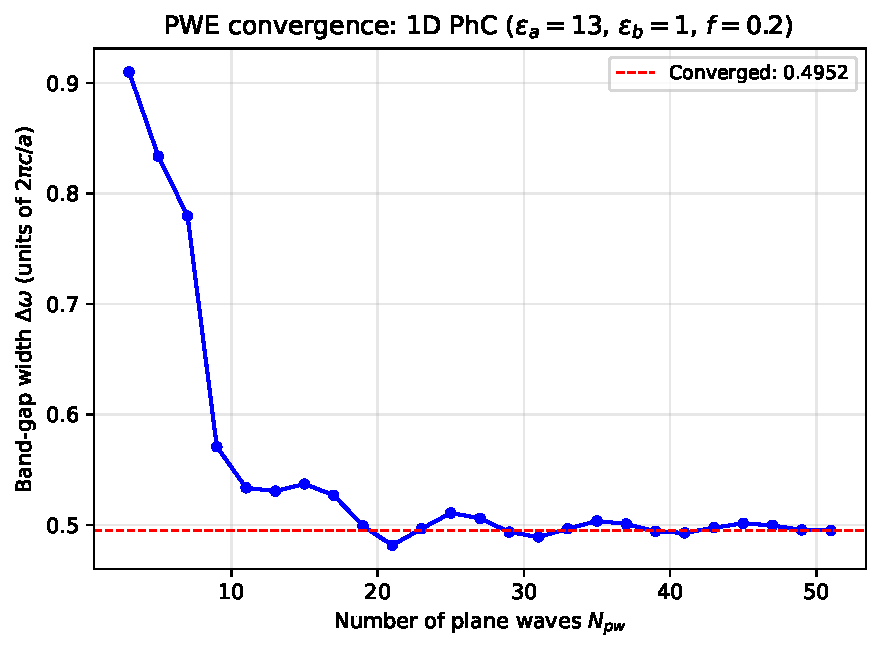
\includegraphics[width=0.6\linewidth]{figures/fig_f03_pwe_convergence.pdf}
 \caption{Convergence of the plane-wave expansion for a 1D photonic
 crystal ($\varepsilon_a = 13$, $\varepsilon_b = 1$, filling fraction
 $f = 0.2$). The computed band-gap width converges rapidly with the
 number of plane waves $N_{\mathrm{pw}}$, reaching the converged value
 $\Delta\omega \approx 0.495$ (in units of $2\pi c/a$) for
 $N_{\mathrm{pw}} \gtrsim 30$ in this one-dimensional test. In higher
 dimensions, sharp high-contrast interfaces usually require more careful
 Fourier factorization and significantly more plane waves.}
 \label{fig:pwe-convergence}
\end{figure}


%% ================================================================
\section{Band gaps}
\label{sec:band-gaps}

A \emph{photonic band gap} is a frequency interval
$[\omega_{\mathrm{low}}, \omega_{\mathrm{high}}]$ in which no Bloch mode
exists for any $\kk$ in the Brillouin zone. The physical consequence is
that light at frequencies within the gap cannot propagate through the
crystal: it is exponentially attenuated, decaying as
$e^{-\kappa(\omega)\,x}$ with a penetration depth set by the imaginary
wave vector $\kappa$.

The existence of a gap requires sufficient dielectric contrast
$\varepsilon_{\max}/\varepsilon_{\min}$ and appropriate lattice geometry. For TM
modes in a 2D crystal of high-$\epsr$ rods in air, gaps open readily;
for TE modes, connected high-$\epsr$ regions (such as air holes in a
dielectric slab) are more favorable.

\paragraph{Perturbative origin of gaps.}
At a Brillouin-zone boundary or high-symmetry point, two bands that would
cross in a uniform medium are coupled by the periodic modulation of
$\epsr$. The resulting level repulsion opens a gap whose width, to
first order in the Fourier coefficient $\hat{\eps}_{\GG}$ of the
relevant reciprocal-lattice vector, is proportional to
$|\hat{\eps}_{\GG}|$. This is the photonic analogue of the
nearly-free-electron picture in solid-state physics.

\paragraph{Variational bounds.}
Since $\Mop_\kk$ is self-adjoint, the Rayleigh quotient provides
variational bounds on the band-edge frequencies. The lowest band satisfies
\begin{equation}
 \frac{\omega_1(\kk)^2}{c^2}
 \le \frac{\int_{\Omega_{\mathrm{uc}}}
 \epsr^{-1}\,|(\nabla + i\kk)\times\mathbf{u}|^2\;\dd^2 r}
 {\int_{\Omega_{\mathrm{uc}}} |\mathbf{u}|^2\;\dd^2 r}
 \label{eq:variational-band}
\end{equation}
for any trial function $\mathbf{u}$, with equality when $\mathbf{u}$
is the exact Bloch eigenfunction. Higher bands are bounded by the
min--max principle. These variational estimates are the theoretical
foundation of the plane-wave expansion method.


\subsection{Field concentration and the physical origin of gaps}
\label{ssec:field-concentration}

The variational principle provides a remarkably intuitive explanation for
why gaps open and which polarization is favored. Consider the two
band-edge modes at a Brillouin-zone boundary where a gap opens. One
mode---the \emph{dielectric band} or lower band edge---concentrates its
electric-field energy in the high-$\epsr$ regions, while the other---the
\emph{air band} or upper band edge---concentrates its energy in the
low-$\epsr$ regions.

The dielectric-band mode has a lower eigenfrequency because the Rayleigh
quotient~\eqref{eq:variational-band} involves $\epsr^{-1}$ in the
numerator: concentrating $|\nabla\times\mathbf{u}|^2$ where $\epsr^{-1}$
is small (i.e., where $\epsr$ is large) reduces the numerator and hence
the eigenvalue. Conversely, the air-band mode is forced to have its curl
energy where $\epsr^{-1}$ is large, raising the eigenvalue. The frequency
difference between these two modes is the band gap.

This field-concentration mechanism explains the TM/TE asymmetry observed
in the 2D example above:
\begin{itemize}
\item \emph{TM modes in rod arrays.} The $E_z$ field is a scalar and
 can concentrate efficiently inside isolated high-$\epsr$ rods. The
 dielectric and air bands have very different field distributions,
 producing a large gap.
\item \emph{TE modes in rod arrays.} The in-plane $\HH$ field must
 satisfy continuity conditions at the rod boundaries that prevent it
 from concentrating entirely inside the rods. The dielectric and air
 bands are more similar, and the gap is small or absent.
\item \emph{TE modes in hole arrays.} When the high-$\epsr$ region is
 connected (air holes in a dielectric slab), the in-plane $\HH$ field
 \emph{can} concentrate in the connected dielectric, and TE gaps open
 readily.
\end{itemize}
A complete photonic band gap---forbidden to both polarizations---therefore
requires a geometry that simultaneously favors both TM and TE gaps, such
as a triangular lattice of air holes with appropriately chosen radius and
dielectric contrast.

The field-concentration picture also explains why gap width increases
with dielectric contrast: larger contrast amplifies the frequency
splitting between modes that concentrate in different materials. This is
precisely the effect captured by the Fourier coefficient
$|\hat{\eps}_{\GG}|$ in the perturbative estimate, which itself grows
with contrast.


%% ================================================================
\section{Degeneracies and symmetry}
\label{sec:degeneracies}

At generic points in the Brillouin zone, the eigenvalues $\omega_n(\kk)$
are non-degenerate. Degeneracies can occur at high-symmetry points where
the little group (the subgroup of the point group that leaves $\kk$
invariant) has irreducible representations of dimension greater than one.

\subsection{Dirac points}
\label{ssec:dirac}

At the $K$ and $K'$ points of a hexagonal Brillouin zone, a pair of bands
may touch linearly, forming a \emph{Dirac cone}~\cite{haldane2008possible,rechtsman2013photonic,khanikaev2013photonic}:
\begin{equation}
 \omega_\pm(\kk) \approx \omega_D \pm v_D\,|\kk - \kk_D| + \cdots,
 \label{eq:dirac-cone}
\end{equation}
where $\omega_D$ is the Dirac frequency and $v_D$ is an effective group
velocity. Near a Dirac point, the two-band effective Hamiltonian takes
the form
\begin{equation}
 H_{\mathrm{eff}}(\delta\kk)
 = v_D\bigl(\delta k_x\,\sigma_x + \delta k_y\,\sigma_y\bigr),
 \label{eq:dirac-hamiltonian}
\end{equation}
with $\sigma_{x,y}$ the Pauli matrices acting on the two-band subspace.
This is the photonic analogue of graphene's electronic Dirac cone.

\subsection{Quadratic touchings and accidental degeneracies}
\label{ssec:quadratic}

At the $\Gamma$ point, symmetry can enforce a quadratic band touching
where $\omega(\kk) \propto |\kk|^2$ rather than $|\kk|$. Perturbations
that break the protecting symmetry can open a gap or split the touching
into a pair of Dirac points.

Accidental degeneracies---those not enforced by symmetry---are generically
avoided in a two-parameter family (the two components of $\kk$ in 2D).
However, they can be tuned by adjusting a third parameter (e.g., the
rod radius or the dielectric contrast). When two bands approach each
other and reconnect, the topology of the band structure can change.


%% ================================================================
\section{Orthogonality and normalization of Bloch modes}
\label{sec:bloch-orthogonality}

The Bloch modes satisfy orthogonality relations that follow from the
self-adjointness of $\Mop_\kk$. For two modes at the \emph{same}
$\kk$,
\begin{equation}
 \int_{\Omega_{\mathrm{uc}}}
 \mathbf{u}_{m\kk}^*(\rr)\cdot\mathbf{u}_{n\kk}(\rr)\;\dd^2 r
 = \delta_{mn},
 \label{eq:bloch-ortho}
\end{equation}
after normalization. For modes at \emph{different} $\kk$ and $\kk'$, the
full Bloch modes $\HH_{n\kk}$ and $\HH_{m\kk'}$ are orthogonal over all
space (or, equivalently, their overlap per unit cell vanishes when
$\kk \neq \kk'$).

This orthonormality is the basis for expanding arbitrary fields in Bloch
modes, defining projection operators onto individual bands, and---as we
shall see in Chapter~\ref{ch:berry-maxwell}---computing the Berry
connection and curvature from the $\kk$-dependence of $\mathbf{u}_{n\kk}$.


%% ================================================================
\section{Group velocity, effective mass, and density of states}
\label{sec:group-velocity-dos}

Beyond the eigenfrequencies $\omega_n(\kk)$, the dispersion surface
contains essential physical information through its derivatives.

\subsection{Group velocity}
\label{ssec:group-velocity}

The group velocity of a Bloch mode is the gradient of the dispersion
relation:
\begin{equation}
 \mathbf{v}_g = \nabla_\kk\,\omega_n(\kk).
 \label{eq:group-velocity}
\end{equation}
It can also be expressed as an expectation value using the
Hellmann--Feynman theorem. Differentiating the unit-cell
eigenproblem~\eqref{eq:unit-cell-evp} with respect to~$\kk$ gives
\begin{equation}
 \mathbf{v}_g
 = \frac{c^2}{2\omega_n}
 \frac{\displaystyle
 \int_{\Omega_{\mathrm{uc}}}
 \mathbf{u}_{n\kk}^*\cdot
 \bigl[
 (\nabla_\kk\Mop_\kk)\,\mathbf{u}_{n\kk}
 \bigr]\;\dd^2 r}
 {\displaystyle
 \int_{\Omega_{\mathrm{uc}}}
 |\mathbf{u}_{n\kk}|^2\;\dd^2 r},
 \label{eq:hellmann-feynman-vg}
\end{equation}
where $\nabla_\kk\Mop_\kk$ is obtained by differentiating the
operator $(\nabla + i\kk)\times[\epsr^{-1}(\nabla + i\kk)\times\,\cdot]$
with respect to~$\kk$. This expression guarantees that the group velocity
is real and bounded whenever $\Mop_\kk$ is self-adjoint.
In non-Hermitian systems, the self-adjointness fails and the group velocity
becomes complex; the physical interpretation of wave-packet propagation
must then be revisited (Chapter~\ref{ch:complex-bands}).

\subsection{Effective mass at band edges}
\label{ssec:effective-mass}

At band edges, where $\nabla_\kk\omega_n = 0$, the band curvature defines
an effective inverse-mass tensor:
\begin{equation}
 (m^{-1})_{ij}
 = \frac{\partial^2\omega_n}{\partial k_i\,\partial k_j}
 \bigg|_{\kk = \kk_0}.
 \label{eq:effective-mass}
\end{equation}
Near a band edge at $\kk_0$, the dispersion is parabolic:
$\omega_n(\kk) \approx \omega_n(\kk_0) + \tfrac{1}{2}\sum_{ij}
(m^{-1})_{ij}\,\delta k_i\,\delta k_j$. This effective-mass
approximation is the photonic analogue of the semiconductor effective mass
and forms the basis for envelope-function theories of photonic-crystal
defect modes and waveguides: a defect introduced into the crystal acts as
a potential well in the envelope equation, binding states pulled out of
the adjacent band edge into the gap.

The effective mass also controls the curvature of the equifrequency
contour near the band edge. An isotropic parabolic band has circular
contours; an anisotropic band has elliptical contours whose principal axes
are aligned with the eigenvectors of $(m^{-1})_{ij}$. In self-collimation
effects, the equifrequency contour is made flat over a range of~$\kk$,
so that wave packets propagate with nearly zero angular spread despite
the discrete lattice.

\subsection{Density of states and van Hove singularities}
\label{ssec:dos}

The \emph{photonic density of states} (DOS) counts the number of modes
per unit frequency. For a two-dimensional photonic crystal,
\begin{equation}
 \rho(\omega)
 = \sum_n \int_{\mathrm{BZ}}
 \delta\bigl(\omega - \omega_n(\kk)\bigr)\;
 \frac{\dd^2 k}{(2\pi)^2}.
 \label{eq:dos}
\end{equation}
(In three dimensions the integration measure becomes
$\dd^3 k/(2\pi)^3$.)
Inside a band gap, $\rho(\omega) = 0$: there are no propagating modes.
This is precisely why spontaneous emission is inhibited in a photonic
band-gap material---the emitter simply has no modes into which it can
radiate.

At band edges, the vanishing group velocity produces \emph{van Hove
singularities} in the DOS. In two dimensions, these are logarithmic
divergences; in three dimensions, they manifest as square-root edges.
Physically, the diverging DOS means that a large number of modes are
compressed into a narrow frequency range, which strongly enhances
light--matter interaction. Slow-light devices, enhanced nonlinear optics,
and low-threshold lasing in photonic crystals all exploit the high DOS
near band edges.

Figure~\ref{fig:ch3-group-velocity-dos} shows the same idea in a simple
model where the geometry is visible at a glance. It is not meant to be a
full plane-wave calculation for a particular dielectric pattern; it is a
teaching model for how stationary points of a dispersion surface become
features of the DOS.

\begin{figure}[t]
 \centering
 
\includegraphics[width=0.94\linewidth]{fig_f3_group_velocity_dos.pdf}
 \caption{Group velocity and density of states in a pedagogical
 square-lattice band model. (a) The colour shows
 $|\nabla_{\kk}\omega|$ and the white curves are constant-frequency
 contours. Stationary points occur at $\Gamma$, at the symmetry-related
 $X/Y$ saddle points, and at $M$. (b) A histogram-smoothed, model-normalized
 DOS in arbitrary units. The dashed lines mark the corresponding band
 bottom, van-Hove saddle feature, and band top. In a full Maxwell band
 calculation the same relation is expressed by
 Eq.~\eqref{eq:dos}: DOS features arise where the dispersion surface has
 small or vanishing group velocity.}
 \label{fig:ch3-group-velocity-dos}
\end{figure}

The local density of states (LDOS), introduced in
Chapter~\ref{ch:light-eigenvalue}, is the position-resolved version of
$\rho(\omega)$ and determines the Purcell enhancement of a dipole emitter
at a given location in the crystal. In the Hermitian case, the LDOS is
non-negative and can be computed from the Bloch-mode expansion. In
non-Hermitian systems (Chapter~\ref{ch:qnm}), the LDOS
must instead be reconstructed from quasinormal modes or from the full
Green tensor. Individual modal contributions can have signs and phases
that have no Hermitian analogue, so only the properly assembled physical
response has the usual positivity properties in passive systems.

\begin{takeaway}[From band diagrams to physical observables]
The photonic band structure is not just a plot---it encodes group
velocity, effective mass, density of states, and through these, the
propagation, confinement, emission, and interaction of light in the
crystal. Every derivative of $\omega_n(\kk)$ carries physical meaning,
and every singularity of the band structure controls a physical effect.
\end{takeaway}


%% ================================================================
\section{Beyond Hermitian bands: a preview}
\label{sec:nh-preview}

The entire construction of this chapter assumed real, positive $\epsr$.
What happens when this assumption is relaxed?

\paragraph{Complex permittivity.}
If $\epsr(\rr) = \epsr'(\rr) + i\epsr''(\rr)$ with the same spatial
periodicity, Bloch's theorem still holds---it depends only on discrete
translational symmetry, not on Hermiticity. But the eigenfrequencies
$\omega_n(\kk)$ become complex, the bands lift off the real axis into the
complex frequency plane, and the orthogonality~\eqref{eq:bloch-ortho}
fails. The ``band structure'' becomes a set of complex-valued curves
$\omega_n(\kk)$, and new topological invariants---winding numbers in the
complex frequency plane---replace the familiar Chern numbers. This is
the subject of Chapters~\ref{ch:complex-bands} and~\ref{ch:point-gap}.

\paragraph{Non-reciprocal media.}
If the permittivity tensor $\epsr(\rr)$ is not symmetric (as in a
magneto-optical medium), time-reversal symmetry is broken and the band
structure loses the constraint $\omega_n(\kk) = \omega_n(-\kk)$. Gaps
can carry nonzero Chern numbers, and topologically protected one-way edge
states appear. This is the domain of topological photonics~\cite{ozawa2018topological,hafezi2013imaging,l2014topological}, developed in
Chapter~\ref{ch:berry-maxwell}.

\paragraph{Open or finite crystals.}
A photonic crystal of finite extent has no exact translational symmetry.
Bloch's theorem does not apply, and the spectrum changes from continuous
bands to a discrete set of resonances. In Hermitian systems, the
bulk-boundary correspondence connects the band topology to the existence
of edge states. In non-Hermitian systems, this correspondence can fail
through the skin effect
(Chapter~\ref{ch:skin-effect}).

\begin{takeaway}[Photonic bands as the Hermitian foundation]
The band structure $\omega_n(\kk)$ of a lossless periodic photonic crystal,
derived from the self-adjoint Maxwell operator acting on Bloch modes in a
unit cell, provides the Hermitian foundation on which all non-Hermitian
photonic band theory is built. Real eigenfrequencies, orthogonal Bloch
modes, variational bounds, and well-defined band gaps are the standard
from which complex bands, point-gap topology, and the skin effect depart.
\end{takeaway}
